\documentclass[tikz,border=2pt]{standalone}
\usepackage{amsmath,amssymb}
\usepackage{tikz}
\usetikzlibrary{matrix}

\begin{document}
% In a canonical tableau the basic variables are the ones whose columns form the identity;
% their values are read directly from the right-hand side.
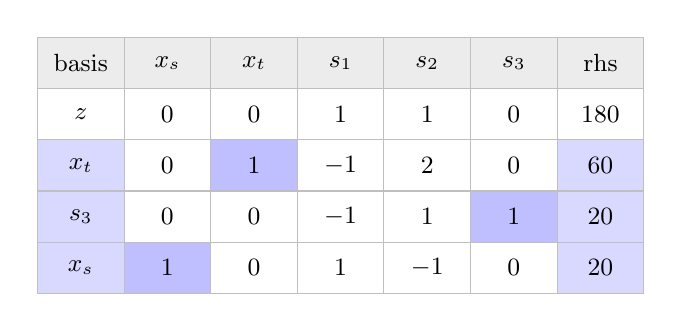
\begin{tikzpicture}[every node/.style={font=\small}]
	\matrix (T) [matrix of math nodes, nodes={minimum width=1.1cm, minimum height=6.5mm, anchor=center, draw=gray!50}, column sep=-\pgflinewidth, row sep=-\pgflinewidth] at (0,0) {
		|[fill=gray!15]| \text{basis} & |[fill=gray!15]| x_s & |[fill=gray!15]| x_t & |[fill=gray!15]| s_1 & |[fill=gray!15]| s_2 & |[fill=gray!15]| s_3 & |[fill=gray!15]| \text{rhs} \\
		z & 0 & 0 & 1 & 1 & 0 & 180 \\
		|[fill=blue!15]| x_t & 0 & |[fill=blue!25]| 1 & -1 & 2 & 0 & |[fill=blue!15]| 60 \\
		|[fill=blue!15]| s_3 & 0 & 0 & -1 & 1 & |[fill=blue!25]| 1 & |[fill=blue!15]| 20 \\
		|[fill=blue!15]| x_s & |[fill=blue!25]| 1 & 0 & 1 & -1 & 0 & |[fill=blue!15]| 20 \\
	};
	\end{tikzpicture}
\end{document}
